\documentclass[aspectratio=169]{beamer}

\usetheme{metropolis}
\title{Лабораторная работа №4: Включение графики и создание перекрестных ссылок в \LaTeX}
\subtitle{Computer Skills for Scientific Writing}
\author{Николаев Дмитрий Иванович, НПМмд--02-24}
\institute{Российский университет дружбы народов имени Патриса Лумумбы}
\date{\today}

\usepackage[utf8]{inputenc}
\usepackage[T2A]{fontenc}
% Исправленный вызов babel для лучшей совместимости с listings
\usepackage[shorthands=off, main=russian]{babel}

\usepackage{graphicx}
\usepackage{listings}
\usepackage{xcolor}
\usepackage{amsmath}
\usepackage{lipsum}
\usepackage{float}

\lstdefinestyle{mystyle}{
    backgroundcolor=\color{black!5},
    commentstyle=\color{green!40!black},
    keywordstyle=\color{magenta},
    stringstyle=\color{purple},
    basicstyle=\footnotesize\ttfamily,
    numbers=left,
    breaklines=true,
    numberstyle=\tiny\color{black!60},
    frame=tb,
    framerule=0pt,
}
\lstset{style=mystyle}

\begin{document}

\frame{\titlepage}

% --- Слайд 1: Цели ---
\section{Цели и задачи}
\begin{frame}{Цель работы}
    \begin{block}{Основная цель}
        Досконально изучить и практически освоить все средства работы с графикой и перекрёстными ссылками в \LaTeX.
    \end{block}
    \begin{alertblock}{Ключевые задачи}
    \begin{itemize}
        \item Воспроизвести все примеры из раздела 4 учебного пособия.
        \item Изучить опции вставки изображений, плавающие окружения и способы их размещения.
        \item Освоить механизм создания перекрёстных ссылок с помощью \texttt{\textbackslash label} и \texttt{\textbackslash ref}.
        \item Исследовать поведение ссылок и изображений в различных условиях.
        \item Создавать кликабельные ссылки в PDF с помощью пакета \texttt{hyperref}.
    \end{itemize}
    \end{alertblock}
\end{frame}

\section{Часть 1: Примеры из пособия}

% --- Слайд 2: Базовая вставка ---
\begin{frame}[fragile]{1.1: Базовая вставка изображения}
    \begin{columns}[T]
        \begin{column}{0.45\textwidth}
            \begin{block}{Код}
            \begin{lstlisting}[language=tex]
\documentclass{article}
\usepackage{graphicx}
\begin{document}
This picture
\begin{center}
  
\includegraphics[height=2cm]
      {example-image.png}
\end{center}
is an imported PDF.
\end{document}
            \end{lstlisting}
            \end{block}
        \end{column}
        \begin{column}{0.55\textwidth}
            \begin{block}{Результат}
            
\includegraphics[width=\linewidth]{image/1.png}
            \end{block}
        \end{column}
    \end{columns}
\end{frame}

% --- Слайд 3: Настройка графики ---
\begin{frame}[fragile]{1.2: Изменение внешнего вида графики}
    \begin{columns}[T]
        \begin{column}{0.5\textwidth}
            \begin{block}{Код}
            \begin{lstlisting}[language=tex]
% --- Scaling ---

\includegraphics
    [height=0.5\textheight]
    {example-image.png}

\includegraphics
    [width=0.5\textwidth]
    {example-image.png}

% --- Cropping ---

\includegraphics
    [clip, trim=0 0 50 50]
    {example-image.png}
            \end{lstlisting}
            \end{block}
        \end{column}
        \begin{column}{0.5\textwidth}
            \begin{block}{Результат}
                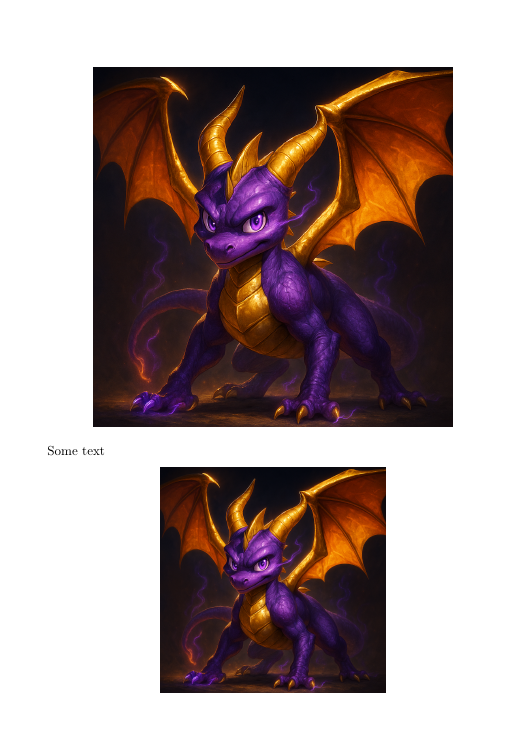
\includegraphics[width=\linewidth, height=0.60\textheight, keepaspectratio]{image/2_1.png}
                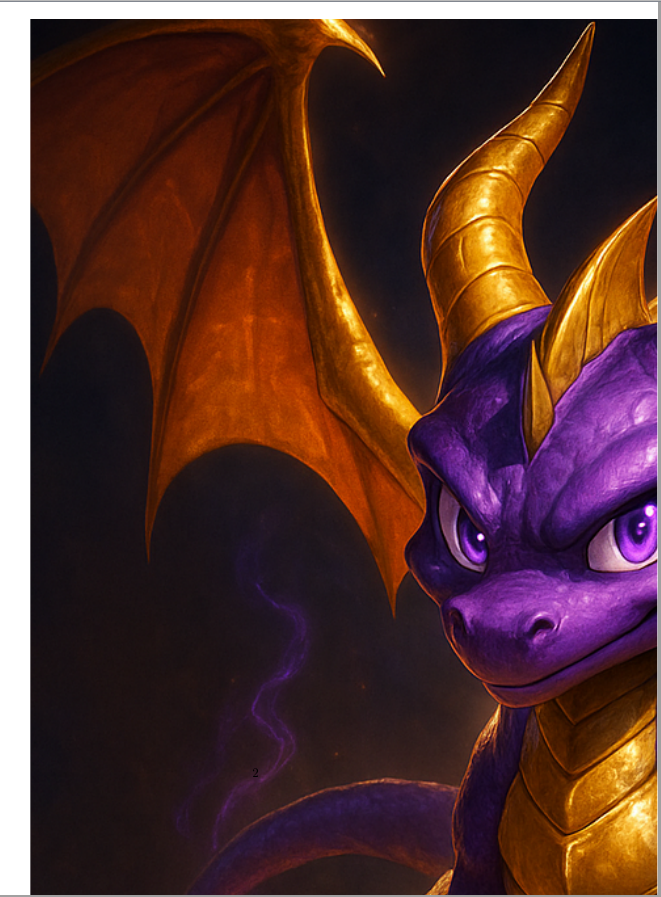
\includegraphics[width=\linewidth, height=0.60\textheight, keepaspectratio]{image/2_2.png}
            \end{block}
        \end{column}
    \end{columns}
\end{frame}

% --- Слайд 4: Плавающие окружения ---
\begin{frame}[fragile]{1.3 \& 1.5: Плавающие и фиксированные окружения}
    \begin{columns}[T]
        \begin{column}{0.5\textwidth}
            \begin{block}{Плавающий рисунок (float)}
            \begin{lstlisting}[language=tex]
\usepackage{lipsum}
%...
\begin{figure}[ht]
 \centering
 \includegraphics{...}
 \caption{An example image}
\end{figure}
            \end{lstlisting}
            \end{block}
            \begin{block}{"Жёсткая" фиксация}
            \begin{lstlisting}[language=tex]
\usepackage{float}
%...
\begin{figure}[H]
...
\end{figure}
            \end{lstlisting}
            \end{block}
        \end{column}
        \begin{column}{0.5\textwidth}
            \begin{block}{Результат}
                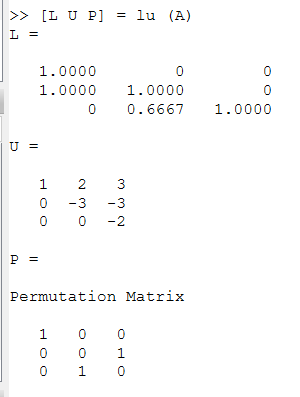
\includegraphics[width=\linewidth, height=0.80\textheight, keepaspectratio]{image/3.png}
                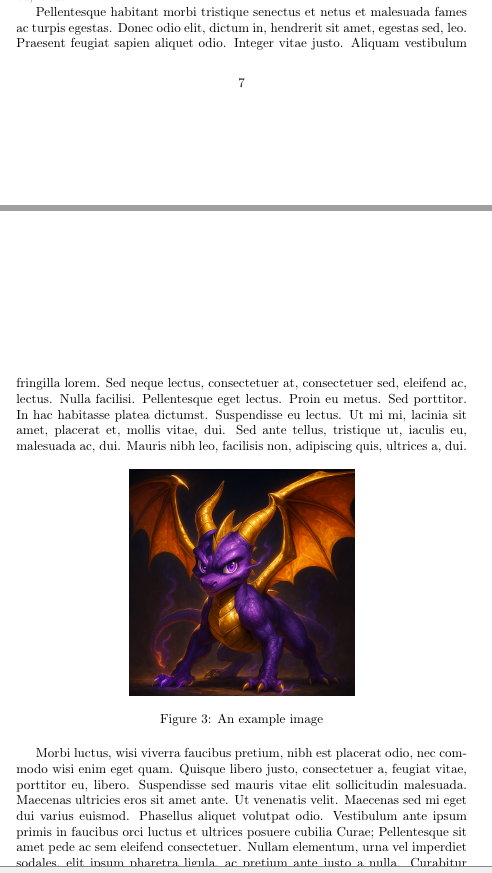
\includegraphics[width=\linewidth, height=0.80\textheight, keepaspectratio]{image/5.png}
            \end{block}
        \end{column}
    \end{columns}
\end{frame}

% --- Слайд 5: Пути и новые окружения ---
\begin{frame}[fragile]{1.4 \& 1.6: Пути к файлам и новые "плавающие" типы}
    \begin{columns}[T]
        \begin{column}{0.5\textwidth}
            \begin{block}{Путь к файлам}
             \begin{lstlisting}[language=tex]
% In the preamble
\graphicspath{{image/}}
%...

\includegraphics[width=0.5\textwidth]{example-image_b.png}
             \end{lstlisting}
            \end{block}
            \begin{block}{Новый тип с \texttt{trivfloat}}
             \begin{lstlisting}[language=tex]
\usepackage{trivfloat}
\trivfloat{image}
%...
trivfloat image
\begin{image}
...
\end{image}
             \end{lstlisting}
            \end{block}
        \end{column}
        \begin{column}{0.5\textwidth}
            \begin{block}{Результат}
                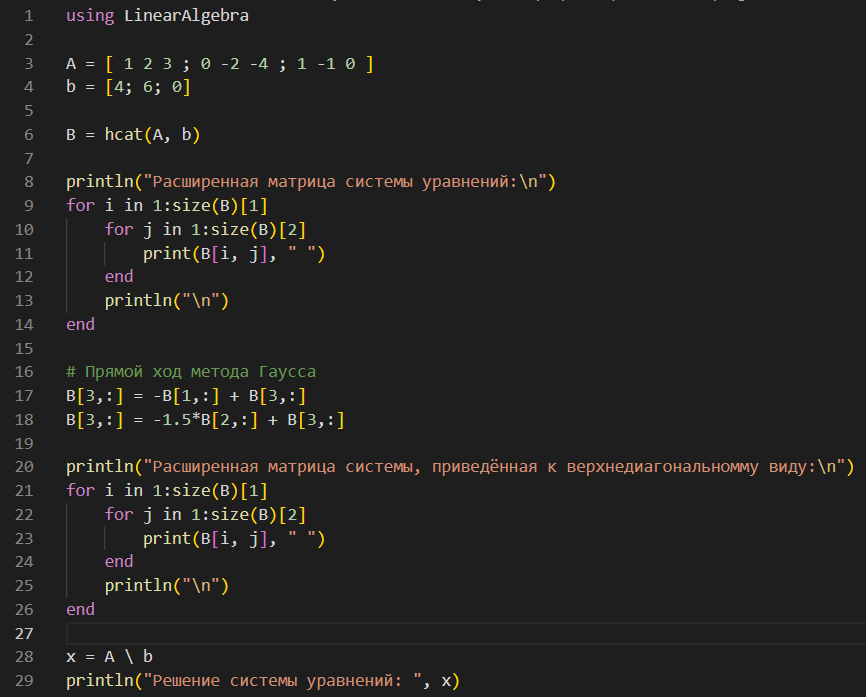
\includegraphics[width=\textwidth, height=0.40\textheight, keepaspectratio]{image/4.png}
                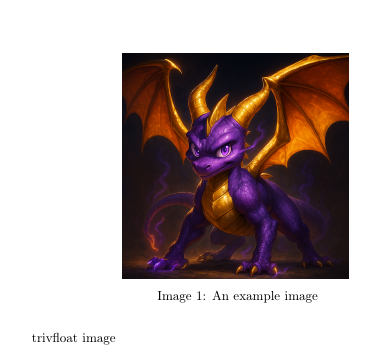
\includegraphics[width=\textwidth, height=0.40\textheight, keepaspectratio]{image/6.png}
            \end{block}
        \end{column}
    \end{columns}
\end{frame}

% --- Слайд 6: Перекрестные ссылки ---
\begin{frame}[fragile]{1.7 \& 1.8: Перекрёстные и гиперссылки}
    \begin{columns}[T]
        \begin{column}{0.5\textwidth}
            \begin{block}{Создание ссылок}
            \begin{lstlisting}[language=tex]
\subsection{My Subsection}
\label{subsec:one}

\begin{equation}
 e^{i\pi}+1=0
 \label{eq:euler}
\end{equation}

Ref to subsec.~\ref{subsec:one}
and equation~\ref{eq:euler}.
            \end{lstlisting}
            \end{block}
            \begin{block}{Кликабельные ссылки}
             \begin{lstlisting}[language=tex]
\usepackage{hyperref}
% All \ref commands become hyperlinks
            \end{lstlisting}
            \end{block}
        \end{column}
        \begin{column}{0.5\textwidth}
            \begin{block}{Результат}
                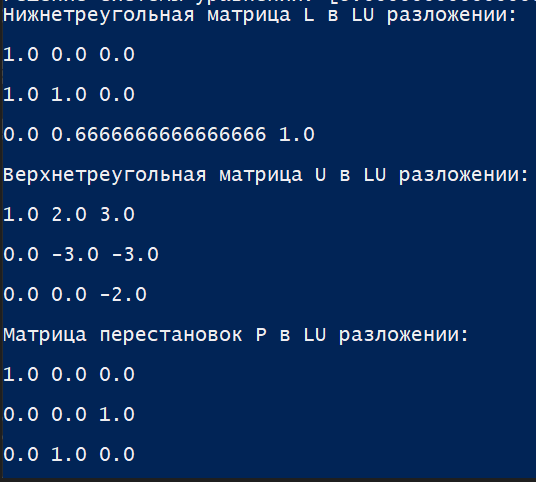
\includegraphics[width=\linewidth, height=0.55\textheight, keepaspectratio]{image/7.png}
                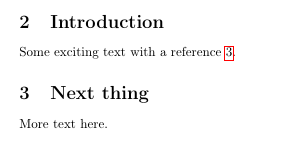
\includegraphics[width=\linewidth, height=0.30\textheight, keepaspectratio]{image/8.png}
            \end{block}
        \end{column}
    \end{columns}
\end{frame}

\section{Часть 2: Итоговые упражнения}

% --- Слайд 7: Упражнения 1-3 ---
\begin{frame}[fragile]{Опции \texttt{figure} и сравнение \texttt{textwidth} vs \texttt{linewidth}}
    \begin{columns}[T]
        \begin{column}{0.5\textwidth}
            \begin{block}{Различные опции \texttt{includegraphics}}
            \begin{lstlisting}[language=tex]

\includegraphics[
  width=0.7\textwidth,
  height=4cm,
  scale=0.8,
  angle=15
]{example-image_b.png}
            \end{lstlisting}
            \end{block}
            \begin{block}{Анализ \texttt{twocolumn}}
                \texttt{\textbackslash linewidth} --- ширина одной колонки, \texttt{\textbackslash textwidth} --- ширина всего текста. Изображение с `width=\textbackslash textwidth` "вылезает" за пределы колонки.
            \end{block}
        \end{column}
        \begin{column}{0.5\textwidth}
            \begin{block}{Результаты}
                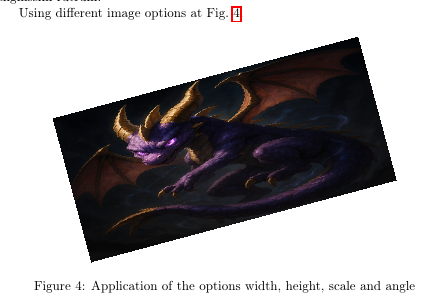
\includegraphics[width=\linewidth, height=0.40\textheight, keepaspectratio]{image/9.png}
                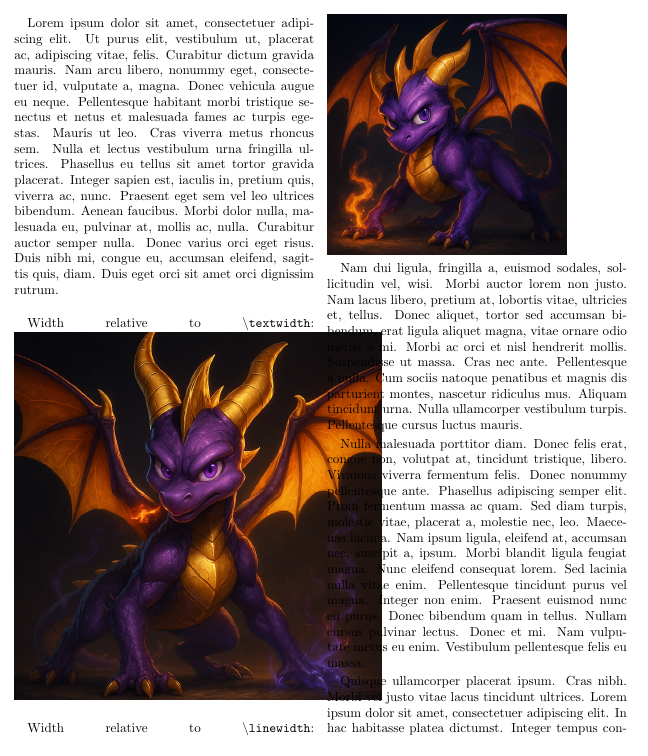
\includegraphics[width=\linewidth, height=0.55\textheight, keepaspectratio]{image/10.png}
            \end{block}
        \end{column}
    \end{columns}
\end{frame}

% --- Слайд 8: Упражнение 4 ---
\begin{frame}[fragile]{Упр. 4: Спецификаторы размещения}
    \begin{columns}[T]
        \begin{column}{0.5\textwidth} \vspace{-3mm}
            \begin{block}{Код эксперимента}
            \begin{lstlisting}[language=tex]
\lipsum[1-3]
\begin{figure}[!htbp]
  \centering
  
\includegraphics
    [width=0.5\textwidth]
    {example-image-c.png}
  \caption{An example image}
\end{figure}
\lipsum[4-5]
            \end{lstlisting}
            \end{block} \vspace{-5mm}
            \begin{block}{Спецификаторы}
            \begin{itemize}
                \item \texttt{h} - here (здесь); texttt{t} - top (вверху)
                \item \texttt{b} - bottom (внизу); page (на отдельной странице)
                \item \texttt{!} - игнорировать ограничения
            \end{itemize}
            \end{block}
        \end{column}
        \begin{column}{0.5\textwidth}
            \begin{block}{Результат с опцией `[!htbp]`}
                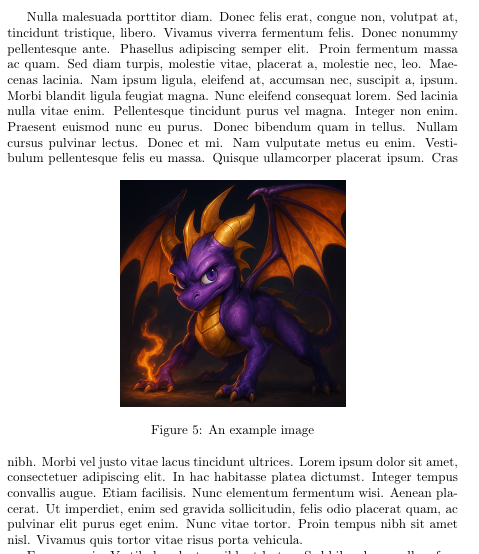
\includegraphics[width=\linewidth, height=0.85\textheight, keepaspectratio]{image/11.png}
            \end{block}
        \end{column}
    \end{columns}
\end{frame}


% --- Слайд 9: Упражнения 5-7 ---
\begin{frame}[fragile]{Упр. 5-7: Важность порядка и расположения \texttt{\textbackslash label}}
    \begin{alertblock}{Ключевой вывод: \texttt{\textbackslash label} запоминает последний обновлённый счётчик.}
       Команда \texttt{\textbackslash label} для рисунка, таблицы или уравнения должна стоять \textbf{ПОСЛЕ} \texttt{\textbackslash caption} или \textbf{ВНУТРИ} нумерованного окружения.
    \end{alertblock}
    
    \begin{columns}[T]
        \begin{column}{0.4\textwidth}\vspace{-3mm}
            \begin{block}{"Неправильный" код}
            \begin{lstlisting}[language=tex]
\begin{figure}[H]
  \label{fig:wrong} % WRONG
  \caption{...}
\end{figure}
Ref: \ref{fig:wrong}
\begin{enumerate}
\label{en:test} % WRONG
\item ...
\end{enumerate}
Ref: \ref{en:test}
\end{equation}
\label{eq:wrong} % WRONG
Ref: \ref{eq:wrong}
            \end{lstlisting}
            \end{block}
        \end{column}
        \begin{column}{0.6\textwidth}
            \begin{block}{Результат: все ссылки указывают на номер подраздела}
                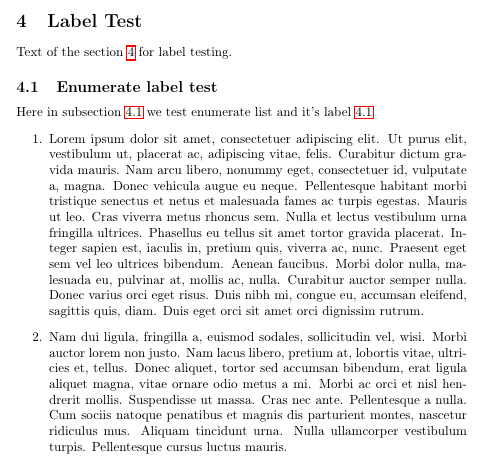
\includegraphics[width=\linewidth, height=0.33\textheight, keepaspectratio]{image/12.png}
                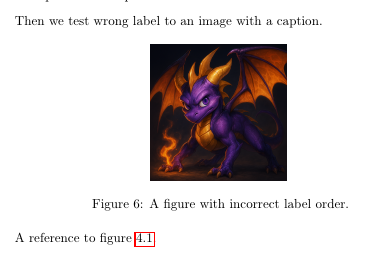
\includegraphics[width=\linewidth, height=0.43\textheight, keepaspectratio]{image/13.png}
                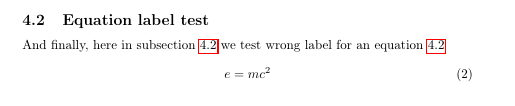
\includegraphics[width=\linewidth, height=0.23\textheight, keepaspectratio]{image/14.png}
            \end{block}
        \end{column}
    \end{columns}
\end{frame}

% --- Слайд 10: Выводы ---
\section{Выводы}
\begin{frame}{Выводы}
    \begin{block}{Освоенные навыки}
    \begin{itemize}
        \item Вставка, масштабирование и кадрирование изображений (\texttt{graphicx}).
        \item Управление расположением графики с помощью плавающих (\texttt{figure}) и фиксированных (\texttt{figure[H]}) окружений.
        \item Организация проекта с выносом изображений в подкаталоги (\texttt{\textbackslash graphicspath}).
        \item Создание надёжной системы перекрёстных ссылок (\texttt{\textbackslash label}, \texttt{\textbackslash ref}).
        \item Понимание критической важности порядка команд и расположения \texttt{\textbackslash label} для корректной нумерации.
        \item Создание интерактивных PDF-документов с кликабельными ссылками (\texttt{hyperref}).
    \end{itemize}
    \end{block}
\end{frame}

\end{document}